%%%%%%%%%%%%%%%%%%%%%%%%%%%%%%%%%%%%%%%%%
% University/School Laboratory Report
% LaTeX Template
% Version 3.1 (25/3/14)
%
% This template has been downloaded from:
% http://www.LaTeXTemplates.com
%
% Original author:
% Linux and Unix Users Group at Virginia Tech Wiki 
% (https://vtluug.org/wiki/Example_LaTeX_chem_lab_report)
%
% License:
% CC BY-NC-SA 3.0 (http://creativecommons.org/licenses/by-nc-sa/3.0/)
%
%%%%%%%%%%%%%%%%%%%%%%%%%%%%%%%%%%%%%%%%%

%----------------------------------------------------------------------------------------
%	PACKAGES AND DOCUMENT CONFIGURATIONS
%----------------------------------------------------------------------------------------

\documentclass{article}

\usepackage[utf8]{inputenc}
\usepackage{graphicx} % Required for the inclusion of images
%\usepackage{natbib} % Required to change bibliography style to APA
\usepackage{amsmath} % Required for some math elements 
\usepackage{glossaries}
\usepackage[toc,page]{appendix}
\usepackage[autostyle=true]{csquotes}
\usepackage{hyperref}
\usepackage{amssymb}
\usepackage{caption} 
\usepackage{hhline}
\usepackage{float}
\usepackage{listings}

\setlength\parindent{0pt} % Removes all indentation from paragraphs

%\usepackage{times} % Uncomment to use the Times New Roman font

%----------------------------------------------------------------------------------------
%	DOCUMENT INFORMATION
%----------------------------------------------------------------------------------------

\title{Specification equals Code:\\An EDSL for pure functional Agent-Based Modelling \& Simulation} % Title
 
\author{Jonathan \textsc{Thaler}} % Author name

\date{\today} % Date for the report

\begin{document}

\maketitle % Insert the title, author and date

% If you wish to include an abstract, uncomment the lines below
\begin{abstract}
Building upon our previous work on update-strategies in Agent-Based Modelling \& Simulation (ABM/S) where we showed that Haskell is a very attractive alternative to existing object-oriented approaches we ask in this paper if the declarative power of the pure functional language can be utilized to write specifications for simple ABM/S models which can be directly translated to our Haskell implementation.
\end{abstract}

\section{Introduction}
There exists a large number of simulation packages which allow the convenient creation of System Dynamics simulations by straight-forward visual diagram creation. One simply creates stocks and flows, connects them, specifies the flow-rates and initial parameters and then runs the model. An example for such a visual diagram creation in the simulation package AnyLogic can be seen in Figure \ref{fig:sir_stockflow_diagram}.

\begin{figure}
	\centering
	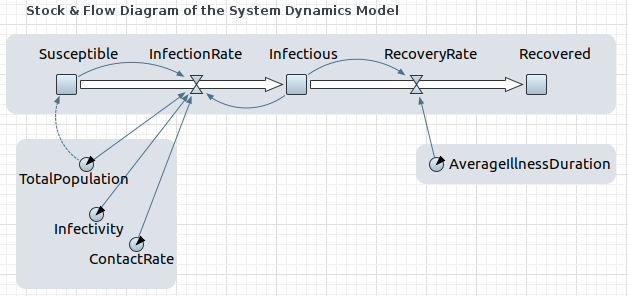
\includegraphics[width=.5\textwidth, angle=0]{./fig/SIR_SD_STOCKFLOW_DIAGRAMM.png}
	\caption{Visual System Dynamics Diagram of the SIR model in AnyLogic Personal Learning Edition 8.3.1.}
	\label{fig:sir_stockflow_diagram}
\end{figure}

Still, implementing System Dynamics directly in code is not as straight forward and involves numerical integration which can be quite tricky to get right. Thus, the aim of this paper is to look into how System Dynamics models can be implemented in code correctly without the use of a simulation package. We use the well known SIR model \cite{kermack_contribution_1927} from epidemiology to demonstrate our approach.

Our language of choice is Haskell because it emphasises a declarative programming style in which one describes \textit{what} instead of \textit{how} to compute. Further it allows to rule out interference with non-deterministic influences or side-effects already at compile-time. This is of fundamental importance for System Dynamics because it behaves completely deterministic and involves no stochastics or non-determinism whatsoever. Also, we make use of Functional Reactive Programming which allows to express continuous-time systems in a functional way. 

We show that by this approach we can arrive at correct-by-construction implementations of System Dynamic models. This means that the correctness of the code is obvious because we have closed the gap between the model specification and its implementation. Thus, the contribution of the paper is the demonstration of how to implement correct-by-construction System Dynamics simulations using Haskell and Functional Reactive Programming.

\section{Related Research}
Already noted in the Introduction, \cite{huberman_evolutionary_1993} where the first to discuss the differences update-strategies can make and introduced the terms of synchronous and asynchronous updates. They define to be synchronous as agents being updated in unison and asynchronous where one agent is updated and the others are held constant.

\medskip

\cite{a_framework_2008} give an approach for ABS on GPUs which is a very different approach to updating and iterating agents in ABS. They discuss execution order at length, highlight the problem of inducing a specific execution-order in a model which is problematic for parallel execution and give solutions how to circumvent these shortcomings. Although we haven't mapped our ideas to GPUs we explicitly include an approach for data-parallelism which, we hypothesize, can be utilized to roughly map their approach onto our terminology. 
	
\medskip
	
\cite{botta_time_2010} sketch a minimal ABS implementation in Haskell which is very similar in the basic structure of ours. This proves that our approach seems to be a very natural one to apply to Haskell. Their focus is primarily on economic simulations and instead of iterating a simulation with a global time, their focus is on how to synchronize agents which have internal, local transition times. Although their work uses Haskell as well, our focus is very different from theirs and approaches ABS in a more general and comprehensive way.

\medskip

\cite{dawson_opening_2014} describe basic inner workings of ABS environments and compare their implementation in C++ to the existing ABS environment AnyLogic which is programmed in Java. They explicitly mention asynchronous and synchronous time-models and compare them in theory but unfortunately couldn't report the results of asynchronous updates due to limited space. They interpret asynchronous time-models to be the ones in which an agent acts at random time intervals and synchronous time-models where agents are updated all in same time intervals.

\medskip

\cite{yuxuan_agent-based_2016} presents in his Master-Thesis a comprehensive discussion on how to implement an ABS for state-charts in Java and also mentions synchronous and asynchronous time-models. He identifies the asynchronous time-model to be one in which updates are triggered by the exchange of messages and the synchronous ones which trigger changes immediately without the indirection of messages.

\medskip

We observe that there seems to be a variety of meanings attributed to the terminology of asynchronous and synchronous updates but the very semantic and technical details are unclear and not described very precisely. In the next section we will address this issue by presenting the basic background and propose properties for a new terminology from which we can derive common update-strategies.

\section{The Problem}

ABM/S is a method of modelling and simulating a system where the global behaviour may be unknown but the behaviour and interactions of the parts making up the system is of knowledge \cite{wooldridge_introduction_2009}. Those parts, called Agents, are modelled and simulated out of which then the aggregate global behaviour of the whole system emerges. Thus the central aspect of ABM/S is the concept of an Agent which can be understood as a metaphor for a unique pro-active unit, able to spawn new Agents, interacting with other Agents in a network of neighbours by exchange of messages which are situated in a generic environment. Thus we informally assume the following about our Agents:

\begin{itemize}
	\item They have a unique identifier
	\item They can initiate actions on their own e.g. change their own state, send messages, create new agents, kill themselves,...
	\item They can react to messages they receive with actions (see above)
	\item They can interact with a generic environment they are situated in
\end{itemize} 

An implementation of an ABS must solve thus solve three fundamental problems:
\begin{enumerate}
	\item Source of pro-activity \\ How can an Agent initiate actions without external stimuli?
	\item Message-Processing \\ When is a message \textit{m}, visible to Agent \textit{B}, processed by it?
	\item Semantics of Message-Delivery \\ When is a message \textit{m}, sent by Agent \textit{A} to Agent \textit{B}, visible to \textit{B}?
\end{enumerate}

In computer systems, pro-activity, the ability to initiate actions on its own without external stimuli, is only possible when there is some internal stimuli, most naturally represented by some generic notion of monotonic increasing time-flow. This can either be some physical real-time system-clock which counts the milliseconds since 1970 (thus binding the time-flow of the system to the one of the 'real-world') or a virtual simulation-clock which is just a monotonic increasing natural number. As we are in a discrete computer-system, this time-flow must be discretized as well in discrete steps and each step must be made available to the Agent, acting as one internal stimuli. This allows the Agent then to perceive time and become pro-active depending on time (NOTE: we could argue that this is not really pro-activity because it depends always on time, but there is really now other way of doing this in our current implementation of computer-systems.). Independent of the representation of the time-flow we have the two fundamental choices whether the time-flow is local to the Agent or whether it is a system-global time-flow.

\medskip 

The semantics of message-delivery define when sent messages are visible to the receivers so they can process them and react to them. The only two ways of implementing them are that messages are visible either \textit{immediately} or after a synchronization point between the sender and receiver. Such a synchronization point can be a local one, just between the two or a global one between all Agents in the system.

\medskip 

Basically we can say that we want to process a message as soon as it is visible to us but this is not how real computer-systems can work. In a real system each Agent would have a message-box into which the messages are posted so the Agent can then check its mail-box for new messages. The question is then when the Agent is going to poll for new messages? Clearly what we need is a recurring, regular trigger which allows the Agent to poll the mail-box and process all queued messages. We argue that the most natural approach is to bind this trigger to the time-flow step which provides pro-activity.

\medskip 

To solve these problems an update-strategy is implemented which will iterate through the Agents in \textit{some} way and allow the Agents to perform these steps. It is immediately clear that different choices in the specific problems will lead to different system behaviour. To discuss this we will first present all possible update-strategies and their details in the next section and then outline how they influence the system behaviour.

\section{The specification Language}

TODO: include environment (continuous, discrete, graph) and position within the environment

introduce environments: discrete, continuous, graph

An Agent A is a 5-tuple <aid, s, m, tf>
aid is the id of the agent
s is the generic state of the agent
m is the message-protocoll the agent understands 


tf is the transformer-function with the following type Agent -> Event m -> Agent



further there is a function for sending a message to other agents
send :: Agent -> (Aid, m) -> Agent

For calculating one iteration of the system we first pair up all agents with the messages they receive in this iteration and then we step every agent
iteration :: [Agent] -> [Agent]
iteration as = stepAll . collectAll

To pair up every agent with all its receiving messages we collect all messages for each single agent
collectAll :: [Agent] -> [(Agent, [(Aid, m)])]
collectAll as = map (\a -> (a, collectFor a as)) as

To pair up a single Agent with its receiving messages, we go over all agents and collect all messages for this current agent
collectFor :: Agent -> [Agent] -> [(Aid, m)]
collectFor a as = foldl (\acc a' -> acc : collectFrom a' aid) [] as
	where
		aid = Aid a

To collect all messages from an agent for a given receiver we simply filter all messages in the outgoing messagebox for the receiving id and then we map the resulting list by replacing the receiving id with the sending id
collectFrom :: Agent -> Aid -> [(Aid, m)]
collectFrom a rid = map (\ (_, m) -> (sid, m)) ms
	where
		sid = Aid a
		ms = filter (\ (rid', m) -> rid == rid') (mbox a)

To step all agents we simply apply step to all agents-message pairs by using map
stepAll :: [(Agent, [(Aid, m)])] -> [Agent]
stepAll = map step

To step an agent we first clear the message-box of the agent, then let consume it its messages and then advance the time 
step :: (Agent, [(Aid, m)]) -> Agent
step = advanceTime . consumeMessages 

TODO: need to clear the message-box but then the elegant function.composition breaks down but this is probably the most elegant play where to do it

Consuming th messages means starting with the initial agent applying the transformation-function for each message resulting in a new agent in every message
consumeMessages :: (Agent, [(Aid, m)]) -> Agent
consumeMessages (a, ms) = foldl tf a ms
	where
		tf = (tf a)

To advance time we simply send the Dt message with the time-step delta to the tranformer-function
advanceTime :: Agent -> Agent
advanceTime a = tf a (-1, Dt 1.0)
	where
		tf = (tf a)

% TODO: the approach

\section{Conclusion and further research}

So far we only looked at recursive simulation in a simulation with a strictly sequential update-strategy where agents are updated in sequence after each other as defined in TODO: cite my Art-Of-Iteration Paper. We leave the question of how Meta-ABS would apply to the parallel update-strategy and whether it is reasonable to extend it to that strategy or not for further research.

Research Questions
\begin{enumerate}
	\item How does deep regression influence the dynamics of a system? Hypothesis: TODO
	\item How do the dynamics of a system change when using perfect information or learning local information? Hypothesis: TODO
	\item Is a hidden markov model suitable for the local learning? Hypothesis: TODO
	\item How can MetaABS best be implemented? Hypothesis: implementing a MetaABS EDSL in a pure functional language like Haskell, should be best suited due to its inherent recursive, declarative nature, which should allow a direct mapping of features of this paradigm to the specification of the meta-model
\end{enumerate}

Problems
\begin{itemize}
	\item Definition of a recursive, declarative description of the Model.
	\item Perfect information about other agents is not realistic and runs counter to agent-based simulation (especially in social sciences) thus an Agent needs to be able to have local, noisy representations of the other agents.
	\item Local representation of other agents could be captured by Hidden Markov Models: observe what other agents do but have hidden interpretation of their internal state - these internal state-representations can be different between the local and the global version whereas the agent learns to represent the global version as best as possible locally.
	\item Infinite regress is theoretically possible but not on computers, we need to terminate at some point
\end{itemize}

\section{Further Research}
\label{sec:further_research}
We see this paper as an intermediary and necessary step towards dependent types for which we first needed to understand the potential and limitations of a non-dependently typed pure functional approach in Haskell. Dependent types are extremely promising in functional programming as they allow us to express stronger guarantees about the correctness of programs and go as far as allowing to formulate programs and types as constructive proofs which must be total by definition \cite{thompson_type_1991, mckinna_why_2006, altenkirch_pi_2010}.

So far no research using dependent types in agent-based simulation exists at all. In our next paper we want to explore this for the first time and ask more specifically how we can add dependent types to our pure functional approach, which conceptual implications this has for ABS and what we gain from doing so. We plan on using Idris \cite{brady_idris_2013} as the language of choice as it is very close to Haskell with focus on real-world application and running programs as opposed to other languages with dependent types e.g. Agda and Coq which serve primarily as proof assistants.

We hypothesize that dependent types could help ruling out even more classes of bugs at compile time and encode invariants and model specifications on the type level, which implies that we don't need to test them using e.g. property-testing with QuickCheck. This would allow the ABS community to reason about a model directly in code. We think that a promising approach is to follow the work of \cite{brady_correct-by-construction_2010, brady_idris_2011, brady_programming_2013, fowler_dependent_2014, brady_state_2016} in which the authors utilize GADTs to implement an indexed monad which allows to implementation correct-by-construction software.

\begin{itemize}
% NOTE: ran out of space
%	\item Accessing the environment in section \ref{sec:adding_env} involves indexed array access which is always potentially dangerous as the indices have to be checked at run-time. Using dependent types it should be possible to encode the environment dimensions into the types. In combination with suitable data types for coordinates one should be able to ensure already at compile time that access happens only within the bounds of the environment.

	\item In the SIR implementation one could make wrong state-transitions e.g. when an infected agent should recover, nothing prevents one from making the transition back to susceptible. 
	
	Using dependent types it should be possible to encode invariants and state-machines on the type level which can prevent such invalid transitions already at compile time. This would be a huge benefit for ABS because many agent-based models define their agents in terms of state-machines.
	
	\item An infected agent recovers after a given time - the transition of infected to recovered is a timed transition. Nothing prevents us from \textit{never} doing the transition at all. 
	
	With dependent types we should be able to encode the passing of time in the types and guarantee on a type level that an infected agent has to recover after a finite number of time steps.
	
	\item In more sophisticated models agents interact in more complex ways with each other e.g. through message exchange using agent IDs to identify target agents. The existence of an agent is not guaranteed and depends on the simulation time because agents can be created or terminated at any point during simulation. 
	
	Dependent types could be used to implement agent IDs as a proof that an agent with the given id exists \textit{at the current time-step}. This also implies that such a proof cannot be used in the future, which is prevented by the type system as it is not safe to assume that the agent will still exist in the next step.

	\item In our implementation, we terminate the SIR model always after a fixed number of time-steps. We can informally reason that restricting the simulation to a fixed number of time-steps is not necessary because the SIR model \textit{has to} reach a steady state after a finite number of steps. This means that at that point the dynamics won't change any more, thus one can safely terminate the simulation. Informally speaking, the reason for that is that eventually the system will run out of infected agents, which are the drivers of the dynamic. We know that all infected agents will recover after a finite number of time-steps \textit{and} that there is only a finite source for infected agents which is monotonously decreasing. 
	
	Using dependent types it might be possible to encode this in the types, resulting in a total simulation, creating a correspondence between the equilibrium of a simulation and the totality of its implementation. Of course this is only possible for models in which we know about their equilibria a priori or in which we can reason somehow that an equilibrium exists.
\end{itemize}

\newpage

\bibliographystyle{acm}
\bibliography{../../references/phdReferences.bib}

\end{document}